% !Mode:: "TeX:UTF-8"
\chapter{引言}
\label{ch:intro}

本章主要介绍了自动驾驶的技术背景以及三维物体检测在自动驾驶技术中的重要作用,然后引出了目前三维物体检测技术的局限性。之后,本章介绍了目前国内外对三维物体检测的研究进展,也简单介绍了三维多目标追踪的研究进展。最后,本章简要概括了本文的工作重点以及技术创新要点,强调了本文研究对于自动驾驶领域的重要意义。

\section{研究背景与意义}
\label{sec:background}
近几年来, 深度学习的迅猛发展赋予了机器越来越强的智能。在计算机视觉、自然语言处理等领域的某些任务上,机器甚至能够表现出比人类更好的性能\cite{he2016deep,DevlinBERT}。 在这样的大背景下, 无人驾驶(Autonomous Driving) 作为最能够体现机器智能的应用场景之一,受到了学术界和工业界的广泛关注。 无人驾驶要求机器能够像人类一样识别道路场景,包括行人和车辆的状态以及车道线等,并且能够根据这些信息高效地进行路径规划来实现与人类类似的驾驶行为。 无人驾驶应用十分广泛,无论是民用还是军工领域。 机器取代人类驾驶车辆,一方面能让人们出行效率更高, 另一方面,机器之间的通讯比人类效率更高,这使得车辆能够更好的规划自己的行驶路径,降低交通事故发生概率。作为智慧城市的不可缺少的组成部分, 无人驾驶也能在非常时期发挥重要作用。譬如在面对重大传染病时(如2019年末爆发的COVID-19),人员之间要尽量减少接触,此时无人驾驶能在保证安全的情况下,极大方便人们的日常生活,包括出行以及货物配送。因此,无人驾驶作为可预见的未来技术,一直是各国在高科技领域的“必争之地”。近十几年来,国内外的无人驾驶平台如雨后春笋般冒出,既有老牌互联网大公司开展的新业务,如国内百度的Apollo\footnote[1]{http://apollo.auto/}(如\figurename \ref{fig:apollo}),美国Google的Waymo\footnote[2]{https://waymo.com/}(如\figurename \ref{fig:waymo})等;也有新型汽车行业巨头,如Uber、特斯拉、滴滴、上汽等;另外,还有新兴的无人驾驶创业公司,如pony.ai、图森未来、驭势科技等。这些都是推动无人驾驶商业化不可忽视的力量,也是推动无人驾驶技术落地的中坚力量。

\begin{figure}[!t]
	\centering
	\begin{minipage}[t]{0.40\textwidth}
		\centering
		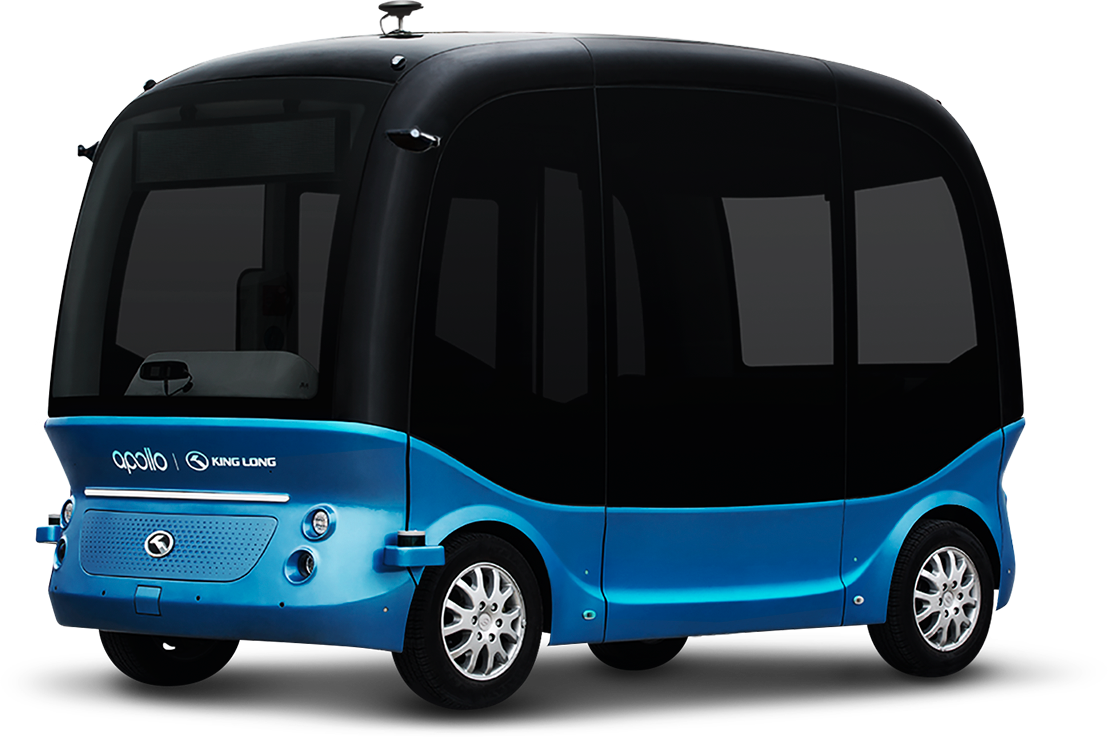
\includegraphics[width=\textwidth]{./imgs/apollo.png}
		\caption{Apollo自动驾驶汽车}
		\label{fig:apollo}
	\end{minipage}
	\begin{minipage}[t]{0.55\textwidth}
		\centering
		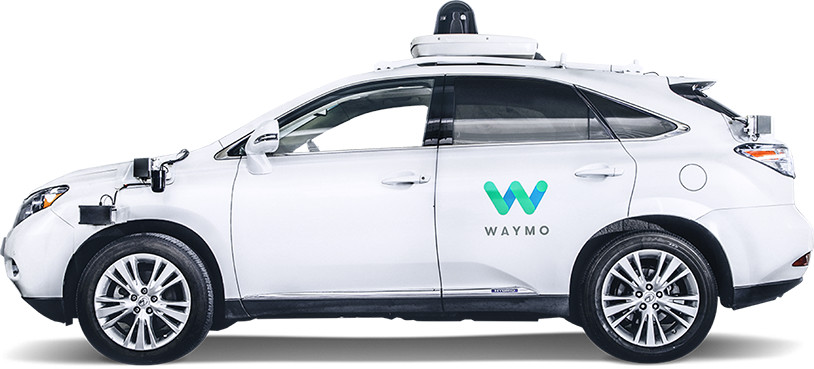
\includegraphics[width=\textwidth]{./imgs/waymo.jpg}
		\caption{Waymo自动驾驶汽车}
		\label{fig:waymo}
	\end{minipage}
\end{figure}


无人驾驶技术主要包括感知、决策和规划三个重要模块,其中感知模块是无人驾驶技术的基础,也是难点。感知模块的任务是赋予机器理解环境的能力,使机器能够准确捕获复杂道路场景的有用信息。目前无人驾驶车辆依赖多种传感器感知环境, 譬如激光雷达(LIDAR)、摄像头、毫米波雷达等。这些传感器都有着各自的优缺点,特别是在价格、使用场景以及探测距离方面,如表\ref{table:sensor_cmp}所示。因此,目前绝大多数自动驾驶公司在感知模块都使用多传感器融合技术,让各传感器优劣互补。多传感器采集的数据会通过算法进行融合,尽可能准确的还原真实的三维环境信息,以便用于后续的目标检测以及跟踪等任务。

环境感知中一大核心任务是物体检测(Object Detection), 即通过分析传感器采集的数据,确定环境中各目标的位姿,包括其在世界坐标系下的坐标、形状信息以及朝向。不同于以图像为主要数据载体的二维物体检测,自动驾驶领域的物体检测任务要求预测目标在三维空间的位姿信息,即三维目标检测。三维目标检测比二维目标检测更加具有挑战性,这是因为维度诅咒(the curse of dimensionality)的存在: 当维度增加时,空间的体积增加的非常之快(以指数增加),以致于可用的数据变得稀疏。 三维物体检测的一大挑战,就是三维数据的稀疏性。目前无人驾驶中三维数据的获得主要是依靠激光雷达,其原理是通过高速旋转的激光发射器向周围发射激光,然后检测接收到反射回来光线的时间间隔来计算反射点的距离。激光雷达的线束对其分辨率有很大影响,特别是对于远距离的目标,在低线束(例如16线)激光雷达中可能只有稀疏的几个点,完全无法分辨。而分辨率高的高线束的激光雷达则十分昂贵,以 Velodyne 64线激光雷达为例,其价格高达十几万美金,因此多数无人驾驶技术方案都需要在激光雷达分辨率与价格之间做出权衡。最近一种非完全旋转的激光雷达——固态激光雷达\footnote[3]{http://www.robosense.cn/rslidar/rs-lidar-m1}受到越来越多人的关注,它们具备数据采集速度快、分辨率高、价格低廉以及环境适应性强等特点,被自动驾驶行业给予厚望。然而目前该技术尚不成熟,还没经过广泛的实际场景检验,离落地还有一段时间,因此暂时不在各大方案的候选传感器之内。短期来看,传统的机械式激光雷达仍是各大自动驾驶平台的首选。

\begin{table}
	\centering
	\wuhao
	\caption{自动驾驶各传感器对比\cite{FirstAVbook}。}
	\vspace{0.3cm}
	\resizebox{\textwidth}{!}{
		\begin{tabular}{cccccccc}
			\toprule[1.5pt]
			传感器    & 激光雷达(LIDAR) & 摄像头(Camera) & 毫米波雷达 \\ \midrule
			外形      & \begin{minipage}{0.13\textwidth}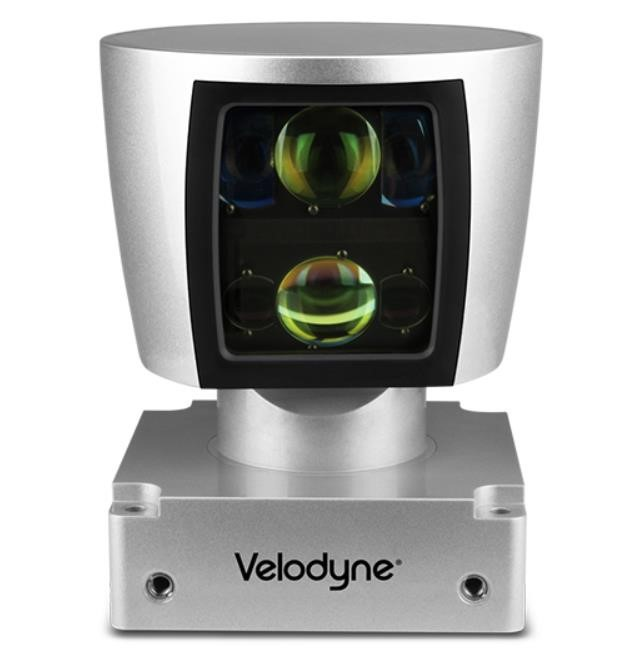
\includegraphics[width=\linewidth]{../figures/imgs/lidar.jpg}\end{minipage} & \begin{minipage}{0.15\textwidth}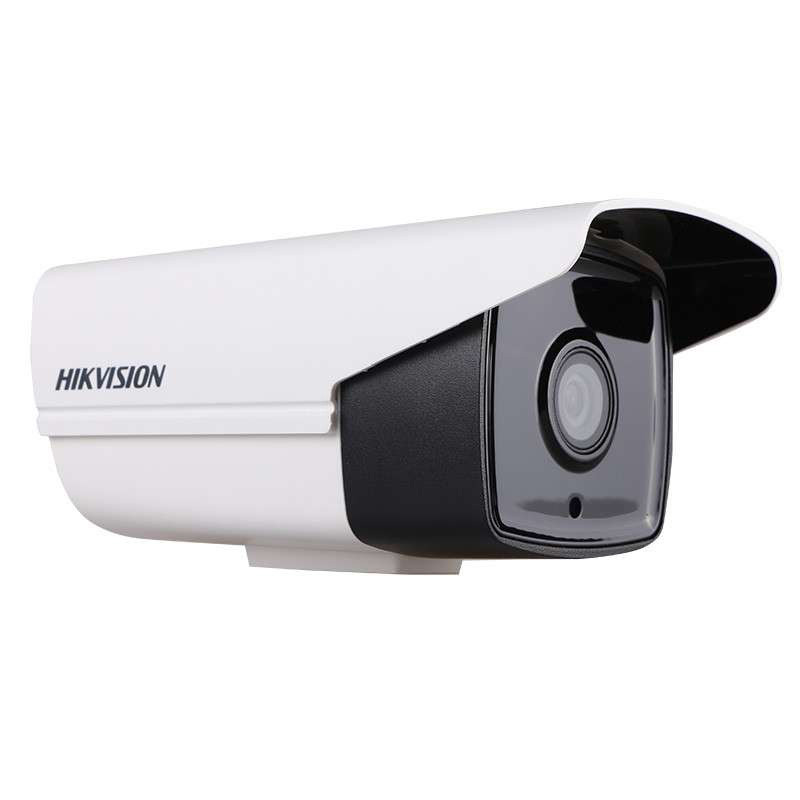
\includegraphics[width=\linewidth]{../figures/imgs/camera.jpg}\end{minipage} & \begin{minipage}{0.15\textwidth}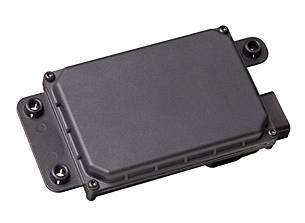
\includegraphics[width=\linewidth]{../figures/imgs/mlidar.jpeg}\end{minipage} \\ \hline
			价格      & 8000美元以上    & 35-50美元         & 300-500美元    \\ \hline
			优点      & \makecell*[c]{扫描周围环境得到精确\\环境信息、距离信息}   & \makecell*[c]{成本比较低,通过算法\\可以实现各种功能} & \makecell*[c]{不受天气影响,\\测量精度高}  \\ \hline
			缺点      & \makecell*[c]{成本高,大雾、雨雪天气\\效果差,无法图像识别}  & \makecell*[c]{恶劣环境下失效,难以测距,\\探测距离较近,算法要求高}   & \makecell*[c]{无法识别道路指示牌,\\无法识别行人}   \\ 
			\bottomrule[1.5pt]
	\end{tabular}}
	\label{table:sensor_cmp}
\end{table}


根据使用传感器数据的不同,目前三维物体检测的研究主要有三个方向:基于图像数据的方案\cite{7780605, chen20183d},基于点云数据的方案\cite{li20173d,engelcke2017vote3deep,zhou2018voxelnet,simon2018complex,shi2019pointrcnn},以及基于多传感器数据融合的方案\cite{qi2018frustum,chen2017multi,ku2018joint}。借助深度学习技术,这些方案都取得了很不错的结果。尽管如此,目前基本所有的三维物体检测方案都是针对单帧数据进行检测。对于真实的自动驾驶场景的物体检测任务来说,数据都是以流的形式连续获取的。从算法落地的难易程度方面考虑,开发针对流数据的三维物体检测算法相比于基于单帧的三维物体检查算法更加具有优势。相比于单帧数据,流数据可以提供同一目标在一段时间内的连续信息。一方面,由于检测噪声(误检测的物体)在时间维度上连续性较差,因此时序上的连续信息有利于检测算法筛除误检测的目标。另一方面,对于遮挡以及物体框被边界截断的目标,在流数据中可以利用前后帧的信息对其进行补全,从而获得更好的检测性能,这对于基于单帧的检测算法来说是难以实现的。最后值得注意的是,流数据一般有很强的数据冗余性,即相邻帧之间绝大多数信息都相同,只有存在物体运动的区域才会有些许差异。对于流数据物体检测,如果使用基于单帧的物体检测算法,则需要逐帧进行检测,然后再将结果关联,这个过程会存在很多重复计算的过程,十分耗时。但是如果使用基于流数据的物体检测算法,则有可能只对少量帧(例如关键帧)进行检测,然后利用流数据的冗余性与时序信息将检测结果传播到其余帧,从而能够更为高效的完成三维物体检测任务。 因此,将基于单帧的三维物体检测算法扩展到流数据场景,能显著提高三维物体检测算法的准确率与效率,也是将三维物体检测技术落实到实际场景的必经之路,具有很强的实践意义。本工作旨在探索基于关键帧的三维流数据物体检测框架,同时也探究了三维时序信息的特征编码以及预测框的传播算法,为后续三维目标检测算法的落地工作提供一个可行的参考方案。

\section{国内外研究进展}
\label{sec:realted_work}
目前国内外针对流数据的三维物体检测研究还较少,而基于单帧数据的三维物体检测以及基于视频流的二维物体检测的研究较为丰富。 因此,本节将简要概述三维物体检测以及视频流物体检测的前沿进展,并分析这些方法的优缺点。另外,本节也将简要介绍三维场景的多目标跟踪的前沿进展,为本工作中多目标跟踪部分提供参考。

\subsection{三维物体检测}
\label{3d_detect}
目前大多数三维物体检测研究可以归类为三大方向:基于图像数据的方案,基于点云数据的方案,以及基于多传感器数据融合的方案,如\figurename \ref{fig:det_algo}所示。基于图像数据的方案中,又可分为基于单目相机数据、基于双目相机数据的三维目标检测;而基于点云数据的方案中根据点云数据的特征提取方式不同又可分为基于点的(Point-based)、基于体素的(Voxel-based)以及基于投影的(Projection-based),这些方法都将在本小节详细介绍。

\begin{figure}[h]
	%\vspace{-0.3cm}
	\begin{center}
		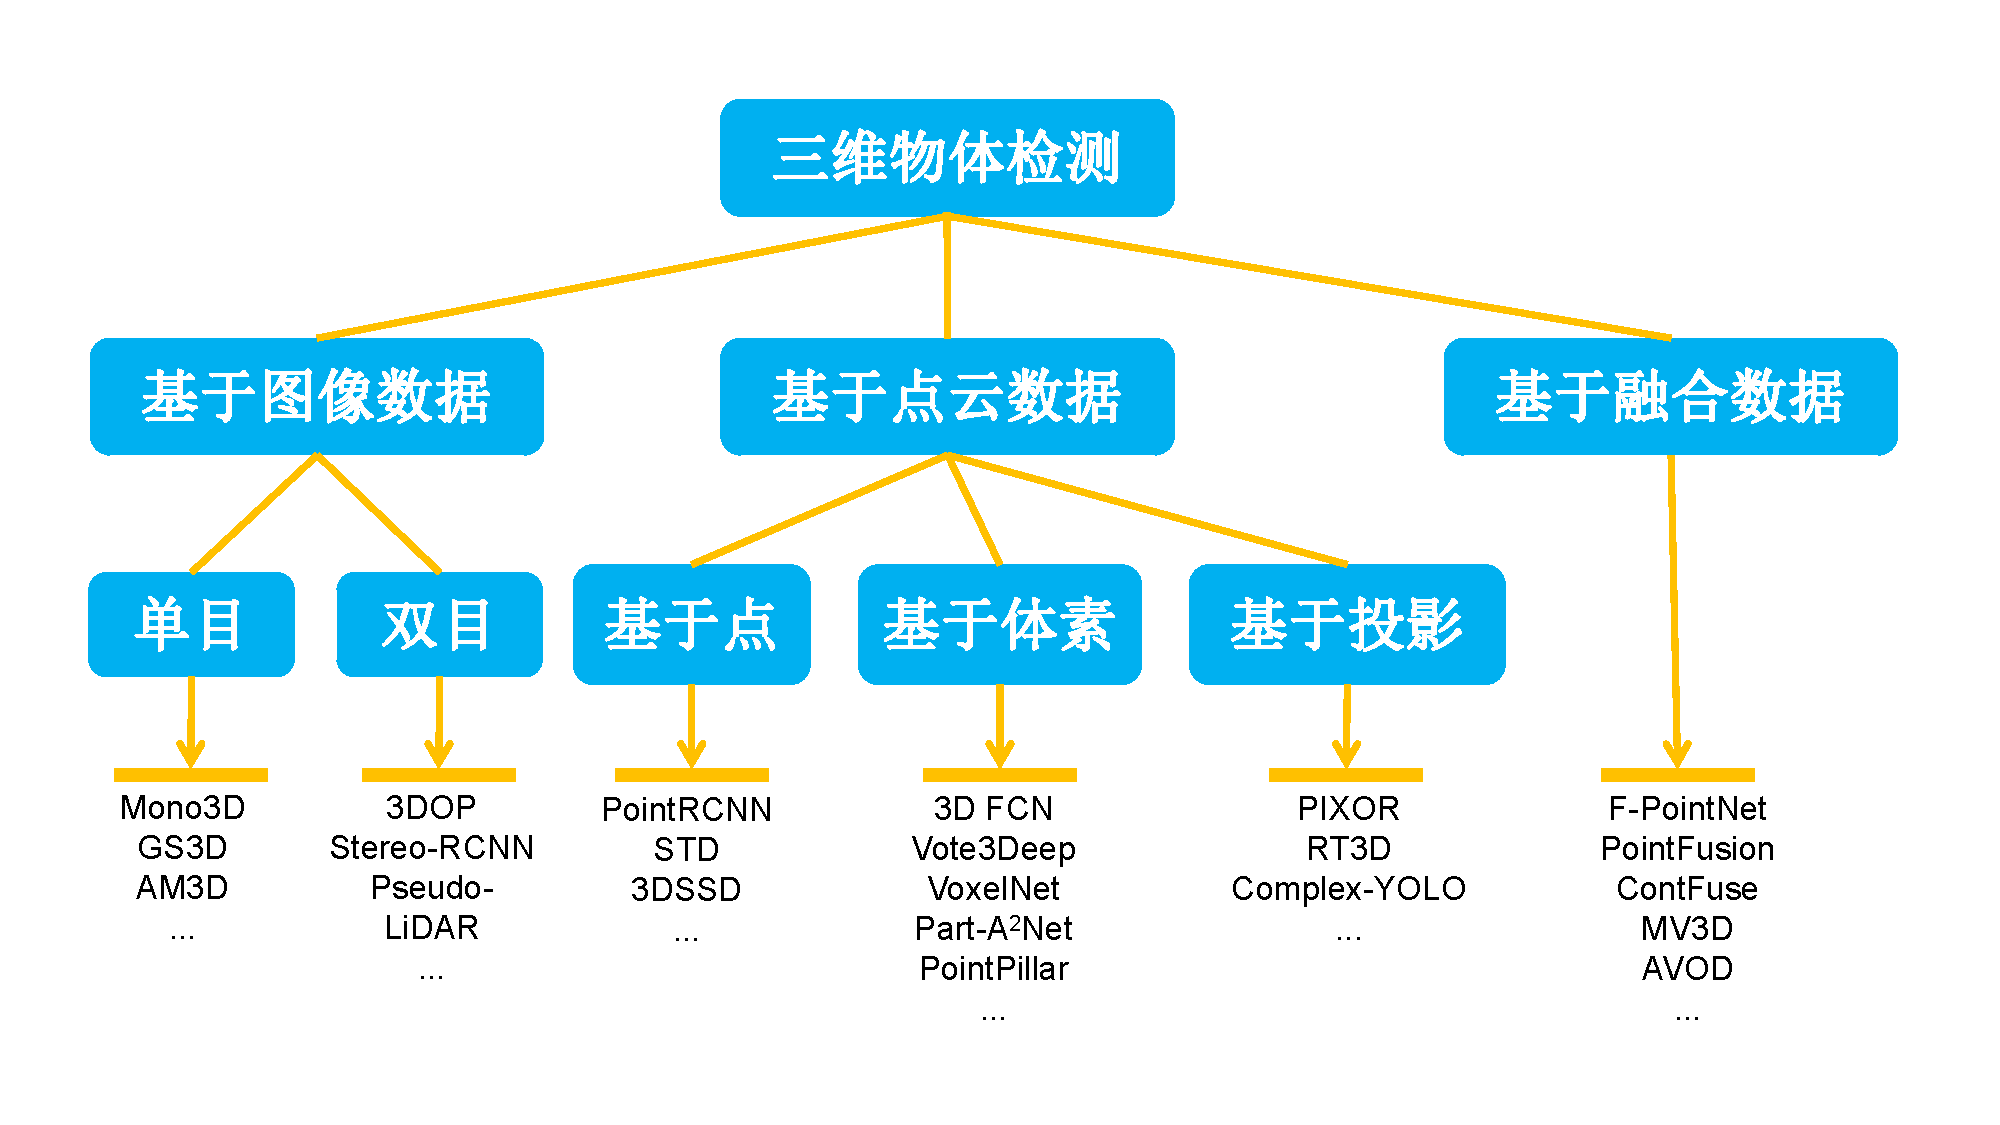
\includegraphics[trim={1.5cm, 1.5cm, 1.5cm, 1.5cm}, clip, width=\textwidth]{imgs/det_algo.pdf}
	\end{center}
	\vspace{-0.8cm}
	\caption{三维物体检测方法分类。}
	\label{fig:det_algo}
\end{figure}


\subsubsection{基于图像数据的三维物体检测}

基于图像数据的三维物体检测有两大类,一类是使用单目摄像头数据,另一类是使用多目(一般为双目)摄像头数据。对于单目摄像头数据,由于摄影几何学的限制,只凭一幅图像是无法恢复出像素点的三维信息的,也无法获得物体的真实的尺寸信息。然而对于特定类型的物体是有可能的,这是因为特定类型的目标往往具有很强的先验信息。这些信息可以被用来构建目标的几何模型,从而使三维物体检测能够顺利进行。对于单目图像三维物体检测,目前有基于目标几何约束提取3D候选框然后将其投影到图像平面提取特征进行预测的,如Mono3D \cite{7780605};也有先对图像进行二维目标检测得到二维边界框,然后利用先验信息对车辆的3D位姿进行建模,从而得到车辆的三维边界框,如\cite{Mousavian3D}以及GS3D\cite{li2019gs3d};另外也有工作使用现有2D物体检测框架以及深度图预测网络得到2D边界框和深度图像,然后再根据相机参数将深度图转换为三维点云,然后利用2D边界框对点云进行分割,最后嵌入RGB信息并使用PointNet\cite{qi2017pointnet}回归出三维边界框,如AM3D\cite{ma2019accurate}。然而,使用单张图像毕竟无法很好地获得物体三维信息,因此这类方法需要人工设计的几何特征来表征物体的深度信息。虽然数据采集简单,速度快,但是检测精度差,落地难。

双目摄像头从生物学上来说很接近人类的双眼视觉系统。对于双目摄像头数据,可以进行双目立体视觉匹配,通过相机之间的相对位置信息可以得到像素点的深度,从而可以在一定程度上恢复物体的三维信息。双目视觉相比于单目视觉有着更强的空间约束关系,因此结合场景先验,可以得到比单目相机更准确的三维物体检测结果。例如,对于两幅成对的图像,3DOP\cite{chen20183d}首先采用了Yamaguchi的方法\cite{Yamaguchi2014Efficient}计算每个像素的深度,生成点云数据,然后采用Struct-SVM\footnote{http://www.cs.cornell.edu/people/tj/svm\_light/svm\_struct.html}优化方法\cite{structSVM}提取3D候选框,最后采用与Fast-RCNN\cite{girshick2015fast}类似框架对3D候选框进行判别和回归,得到最终的预测框。Stereo RCNN\cite{licvpr2019}则将Faster-RCNN\cite{ren2015faster}网络扩展到双目立体视觉,将左右图像输入两个相同的候选框提取网络,然后通过自动对齐学习计算出左右视图中匹配的候选框,最后通过稠密匹配优化得到最终的三维检测结果。此外,还有工作使用双目相机数据生成伪激光雷达数据,然后使用这些点云数据进行三维物体检测。伪激光雷达数据的生成一般使用的是DRON\cite{DRON}或PSMNET\cite{chang2018pyramid}等深度估计网络,这类方法的代表是Pseudo-LiDAR\cite{Wang_2019_CVPR,you2020pseudolidar}。不过双目视觉对于远处的像素点深度估计非常不准,并且存在盲区,因此基于双目视觉的三维物体检测方案存在自身的理论缺陷,只能依靠神经网络根据先验信息弥补系统误差。

\subsubsection{基于点云数据的三维物体检测}

基于点云数据的方案是三维物体检测的主流方向,根据点云数据的特征提取方式不同这些方法又可分为Point-based、Voxel-based 以及Projection-based,本小节将详细介绍这三类方法。

Point-based的方法是直接在点云中提取特征,可以使用PointNet\cite{qi2017pointnet}, PointNet++\cite{qi2017pointnet++}, PointCNN\cite{PointCNN}, PointSIFT\cite{JiangPointSIFT}, Octnet\cite{RieglerOctNet}, Dynamic Graph CNN\cite{WangDynamic}等方法提取点的特征。Point-based的方法中比较有代表性的是香港中文大学提出的PointRCNN\cite{shi2019pointrcnn}以及其后续工作STD\cite{std2019yang}和3DSSD\cite{yang3DSSD20}。PointRCNN方法分为两步,第一步是将整个场景的点云分割为前景点和背景点,然后以自下而上的方式生成高质量候选框;第二步是将每个候选框进行坐标规范化,以便更好的学习局部空间特征然后生成更精确的边界框。STD在此基础上提出了一种基于球形锚点框的点云候选区域提取网络,然后引入了新的点池化层将候选区域内部点的特征从稀疏表达转化为稠密表达。相比于PointRCNN,STD具有更高的召回率以及更少的计算量。3DSSD是同一个研究团队提出的更加轻量型的单阶段三维物体检测网络,该网络提出了一种新的融合采样策略替代之前的上采样层,能够在准确率和速度上达到很好的平衡。这些方法在点云特征提取上都借鉴了PointNet++的思想,特别是使用\textit{set abstraction}操作在点云特征提取中引入可变的感受野。

Voxel-based的方法使用三维体素网格编码点云特征, 每个体素立方体的值由该立方体内的点决定,从而将不规则的三维点云数据编码成规则的三维体素数据, 便于后续使用神经网络进行特征提取。 这方面的代表工作有 3D FCN \cite{li20173d}、Vote3Deep \cite{engelcke2017vote3deep}、 VoxelNet \cite{zhou2018voxelnet}、Part-$A^2$Net\cite{shi2020part}以及PointPillar\cite{lang2018pointpillars}等。3D FCN和Vote3Deep直接对网格化的点云数据使用3D卷积提取特征,由于点云非常稀疏并且3D卷积需要在三个维度上操作,因此整个检测、定位的过程极其耗时。此外,受到感受野的影响,传统的3D CNN并不能很好的学习不同尺度的局部特征。VoxelNet只对非空的网格进行特征提取,并且使用多尺度结构学习不同尺度的信息,一定程度上弥补了这类方法的劣势。Part-$A^2$Net直接引用了VoxelNet的体素化方法,使用了稀疏卷积以及子流型稀疏卷积(Submanifold Sparse Convolution\cite{Graham3D})提取点云特征。PointPillar则是提出新型的垂直柱体网格化方法编码点云特征,使得编码速度更快。这类方法的一大缺点是体素大小不好确定,太大的话信息损失严重,太小则会造成巨大的计算量。 

Projection-based的方法是将点云在高度方向进行投影,将三维数据降维成二维的俯视图(BEV, bird eye view)数据。 考虑到在驾驶场景中, 道路基本是共面且水平的,因此在高度方向上投影对物体的位姿信息基本没有损失。 经过投影操作后,就能直接使用二维图像物体检测的方法进行物体检测。 PIXOR \cite{yang2018pixor}、RT3D\cite{8403277} 以及 Complex-YOLO \cite{simon2018complex,Simon_2019_CVPR_Workshops} 等属于这类方法,这些方法主要不同点在于点云的投影视角以及投影方式。 虽然降维能够带来速度的极大提升,然而由于点云数据的稀疏性,经过投影后目标的特征点损失很严重。 特征点的不足会很大程度上影响检测结果的准确性,特别是对于远处的目标以及小目标。

\subsubsection{基于多传感器数据融合的三维物体检测}

点云的稀疏性以及图像缺少深度信息都限制着相应方法的性能,一个自然而然的想法就是将这两种数据融合, 从而达到更好的检测性能。 基于多传感器融合的方法通过算法融合点云数据以及图像数据,从而提升三维物体检测的准确率。 这类方法的代表有 F-PointNet \cite{qi2018frustum}、PointFusion\cite{XuPointFusion}、ContFuse\cite{Ming2018Deep}以及 MV3D \cite{chen2017multi}、AVOD \cite{ku2018joint}等。 这些方法的区别主要在于数据融合的方式不同, F-PointNet首先使用二维物体检测方法检测出图像中的所有物体,之后对于每个物体,将其反投影回点云中得到一个视锥区域,之后使用PointNet++\cite{qi2017pointnet++}对该区域内的点进行分割,最后进行框回归。该方法通过先在图像中找出目标的大致区域,从而减少了算法在点云空间的搜索空间。然而,该算法的准确率受二维物体检测精度影响很大,在第一步没有检测出的物体,之后没有其他办法弥补。 PointFusion和ContFuse都是先分别在图像与点云数据中使用网络提取特征,然后将这两类特征进行融合并实现三维物体检测。MV3D 则是将二维物体检测中的区域提取网络扩展到三维空间, 提出了三维特征提取网络分别提取点云以及图像特征, 然后通过一个特征融合模块得到多视角融合特征,最后基于融合特征进行三维物体检测。 AVOD 在 MV3D 的基础上改进了特征提取模块, 引入了编码器-解码器结构从而能够得到全分辨率的特征图, 重点提升了小物体的定位精度。 本文工作中的检测模块是在AVOD框架的基础上进行改进的,使其能支持多帧输入,并引入了时序信息处理模块融合连续帧信息。

\subsection{视频流物体检测}
\label{video_detect}
视频流物体检测与单帧物体检测的主要区别在于是否利用了时序信息。 对于视频流物体检测而言,时序信息是物体的位姿在时间上连续性的抽象体现。 目前,大多数视频流物体检测方法都是在两个层面利用时序信息,特征提取层面以及最终的边界框回归层面。 对于特征处理层面, 一般是根据运动信息将前后帧的的特征整合到关键帧,以丰富关键帧中物体的特征。 这个过程中需要使用到光流信息,即图像中各像素点的运动信息,该方向的代表有 FGFA \cite{zhu2017flow}系列工作。 一般来说光流信息的获取是比较困难的,这也是限制这一类方法进一步发展的主要障碍。 对于在边界框回归层面利用时序信息,主要的工作有 T-CNN \cite{kang2018t, kang2016object} 与 Seq-NMS \cite{han2016seq}等。 T-CNN 使用预先计算的光流信息将关键帧的检测结果传播到临近帧,而 Seq-NMS 则是通过整合连续几帧的高置信度的候选框来提升目标检测中非极大值抑制算法的性能。 最近, 也有一些工作试图通过神经网络学习连续帧之间的的时序信息, 从而避免使用高代价的光流数据。 这类方法的代表有 D\&T \cite{feichtenhofer2017detect}。 D\&T 提出了一个双路目标检测网络,可以同时实现视频流的目标检测以及目标追踪。 该网络可以输入多帧数据进行检测, 并且通过互相关操作(Cross-correlation) 来学习相邻帧之间相同物体的对应关系以及位置偏移。 本工作的网络框架在一定程度上也借鉴了 D\&T 的结构, 不过我们在它的基础上进行了很大的改进,使其能够适应三维空间的流数据物体检测。

\subsection{三维多目标追踪}
\label{tracking}
目前基本上所有的三维多目标追踪方法都是先对流数据的每一帧进行目标检测,然后再将这些检测框关联起来, 这种方法也被称为 \textit{Tracking by Detection} \cite{lenz2015followme}模式。 三维多目标追踪的工作有很多,比较有代表性的有 FaF \cite{luo2018fast}, 3D-CNN/PMBM \cite{scheidegger2018mono}以及 DSM \cite{frossard2018end}等。 FaF 使用首先将点云流数据结构化成四维张量,然后构建了一个简单的特征提取网络提取特征,最后使用不同的网络头分别预测得到三维目标检测、多目标追踪以及物体运动方向预测结果。该方法能够整合前 $n$ 帧的检测结果得到更精确的物体运动轨迹。 然而该方法计算量巨大, 并且网络参数调节需要很高的技巧。  3D-CNN/PMBM 首先构建神经网络从单张图像预测物体的三维位姿, 然后将所有帧的检测框送入泊松多重伯努利 (Poisson Multi-Bernoulli Mixture, PMBM) 混合追踪滤波器进行滤波,得到最终的三维多目标追踪结果。 该方法只使用单帧图像进行三维目标检测,效果有限。 DSM 首先使用单帧三维物体检测框架 MV3D \cite{chen2017multi} 对每一帧数据进行物体检测得到三维检测框, 然后通过一个匹配网络(\textit{Matching net})以及得分网络(\textit{Scoring net})关联所有的检测框。 该方法需要对每一帧数据进行检测, 无法有效利用帧与帧之间的时序信息,因此不是针对流数据的高效追踪方法。

\section{本文工作及创新点}
\label{subsec:contribution}
本文创新性的提出了一个双路物体检测与追踪(\textbf{D}ual-way \textbf{O}bject \textbf{D}etection and \textbf{T}racking, \textbf{DODT})框架, 实现了流数据场景的高效三维物体检测与追踪。 DODT框架的构建是基于以下几个观察: (1) 点云数据能够与图像数据融合从而丰富物体的视觉特征, 这点在 \cite{chen2017multi,ku2018joint}中得到了证实; (2) 除了通过光流数据, 时序信息也能够通过计算相邻帧间的互相关信息,这点通过 D\&T\cite{feichtenhofer2017detect} 也能够得到验证; (3) 特征在连续帧之间的变化是连续的, 我们可以只对关键帧进行检测,然后将结果传播到非关键帧, 这样可以极大的减少计算量。 对于第一点, 本文借用了 AVOD\cite{ku2018joint} 中的数据融合方案,将点云数据的 BEV 视图信息与图像数据融合。 对于第二点, 本文构建了一个时序信息处理模块(Temporal module), 该模块使用互相关操作(Cross-correlation)在 点云数据的BEV视图空间中计算相邻关键帧的时序特征, 然后预测相同物体在两关键帧中同时出现的概率以及对于的位姿偏移量。 与 \cite{feichtenhofer2017detect,dosovitskiy2015flownet} 不同的是, 本模块的互相关操作是在候选框层面上进行的,不需要针对全局进行搜索计算, 这极大地提高了互相关信息的提取效率。 对于最后一点, 我们将 DODT 框架的目标检测模块设计成了双路结构。 这样该模块就能够同时输入两帧相邻关键帧数据,并且实现只对关键帧数据进行预测然后将结果传播到非关键帧,此外这也保证了时序信息处理模块的正常运行。 另外, 为了进一步提高框架的运行效率, 本文还设计了一个共享 RPN (Shared Region Proposal Network, Shared RPN) 模块, 该模块可以生成供两检测分支共同使用的三维候选框。 最后,为了生成所有帧的检测结果, 本文设计了一个基于运动模型的框插值算法, 该算法利用关键帧的检测结果以及时序模块预测的信息,插值生成非关键帧的检测结果。 同时, 该插值算法还能够将不同帧的物体边界框关联起来, 得到三维物体的多目标追踪结果。

综上所述,本文的贡献及创新点列举如下:
\begin{itemize}
	\item 本文提出了一个名为 DODT 的双路检测网络, 该网络能够同时精确地完成流数据的三维物体检测以及多目标追踪任务。
	\item 本文提出了一个时序信息模块,能够在候选框层面编码相邻关键帧之间的时序信息。 相比于\cite{feichtenhofer2017detect,dosovitskiy2015flownet}中方法, 该方法更加灵活,也更加高效。
	\item 本文设计了一个共享 RPN 模块, 该模块能够显著提高相邻多帧在目标检测中候选框提取的效率。
	\item 本文开发了一个基于运动模型的框插值算法, 该算法能够有效的将关键帧的预测框传播到非关键帧, 同时也能够高效的将所有物体边界框关联起来, 实现三维多目标追踪。
\end{itemize}


\section{文章组织与结构}
\label{subsec:structure}
本文的主要内容分为五章。 第一章为引言, 介绍项目的研究背景和意义, 国内外的研究进展以及本文工作的简单介绍和创新点; 第二章介绍本工作涉及到的一些技术的基础理论, 分为目标检测与目标追踪两大块; 第三章详细地介绍了本文提出的DODT框架的构造和原理, 是全文的重点内容; 第四章主要介绍了本项目的实验设计、实验结果分析以及结果展示, 该部分也是全文的重点内容; 最后一章总结本文的工作, 然后介绍本文工作的不足之处以及后续的研究方向。 


% 打印时插入必要的空白页
\ifprint
	\newpage
	\thispagestyle{empty}
	\mbox{}
	
	% 避免空白页影响页码编号
	\clearpage
	\setcounter{page}{10}
\fi